\section{Physical Simulation}

Physically-based character animation consists of two parts, simulation and control. This section concentrates on the simulation part while the next section on control. Although the majority of research in physically-based character animation focuses on control, a good understanding of physical simulation is essential for designing effective controllers because complex human behaviors often require sophisticated controllers that exploit the dynamics of a multi-body system.

\begin{figure}[h]
  \centering
  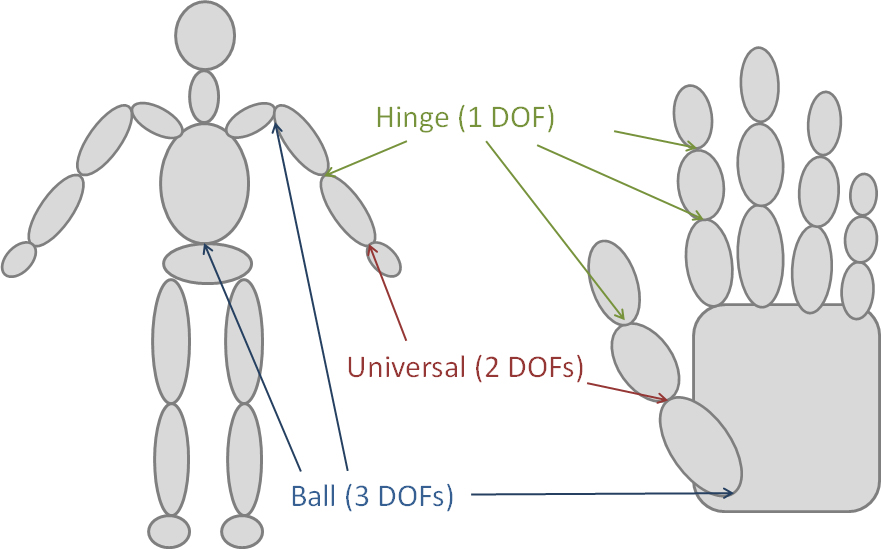
\includegraphics[width=0.6\textwidth]{figures/character.jpg}
  \caption{Articulated figures in character animation to represent a human character (left) and a hand (right).}
  \label{fig:character}
\end{figure}

In physically-based character animation, a human character is often represented as an articulated rigid body system (Figure \ref{fig:character} left), a group of rigid bodies chained together through rotational joints. These joints can have different number of degrees of freedom (DOF). For example, the shoulder is a ball joint (3 DOFs), the wrist is a universal joint (2 DOFs) and the elbow is a hinge joint (1 DOF). In some cases, if the character's motion involves dexterous hand manipulation, a detailed hand model (Figure \ref{fig:character} right) is attached to each wrist. Note that this human model is a dramatic simplification since simulating each bone, muscle and tendon that a real human has would require a prohibitively huge amount of computational resources. In the simulation, the articulated figure is represented as a tree structure. A node is a rigid body and each edge is a joint. Each node can have multiple children but at most one parent. The root node has no parent. Any body can be selected as the root node, but a common practice is to use the torso as the root. In this tree representation, loops are not allowed. Although it is possible to simulate loops, such case is rare in character animation and will not be discussed here. There are two major methods to simulate the dynamics of an articulated rigid body system. It can be simulated in maximal coordinates (Cartesian space) or in generalized coordinates (joint space).



\subsection{Simulation in Maximal Coordinates}

In maximal coordinates, the physical states of the articulated figures are defined for each node (rigid body). Each body has six degrees of freedom: three translational and three rotational. The dynamics of each rigid body is considered independently. A list of additional joint constraints is imposed to ensure that the two adjacent bodies will stick together at the joint location. The dynamics equation for each body is 

\begin{equation}
\left[\begin{array}{cc}
m\vc{I}_{3\times3} & \vc{0} \\
\vc{0} & \vc{I}
\end{array}\right]
\left[\begin{array}{c}
\dot{\vc{v}} \\
\dot{\vc{\omega}}
\end{array}\right]=
\left[\begin{array}{c}
m\vc{g} \\
-\dot{\vc{I}}\vc{\omega}
\end{array}\right]
+\left[\begin{array}{c}
\vc{f}\\
\boldsymbol{\tau}
\end{array}\right]
+
\left[\begin{array}{c}
\vc{0}\\
\boldsymbol{\tau}^a
\end{array}\right]
\label{eq:dynamics}
\end{equation}
where $m$ and $\vc{I}$ are the mass and the inertia tensor of the body. $\vc{I}_{3\times 3}$ is a $3\times 3$ identity matrix. $\vc{v}$ and $\vc{\omega}$ are the linear and angular velocities. $[\vc{f}, \boldsymbol{\tau}]^T$ are the passive forces and torques from joint constraints, contacts, gravity and other external sources. $\boldsymbol{\tau}^a$ are the torques actively exerted by the controllers, which is the focus of Section 4.

Joints that connect two rigid bodies constrain their relative motions. Different number of constraints is imposed according to the type of joints. For example, a hinge joint has only one DOF. Thus it has five constraints that eliminate all but the rotation along the hinge axis. A ball joint has three DOFs. Its constraints eliminate the relative translation at the joint location. 

Suppose a joint connects body $A$ and body $B$, the translational constraints are:

\begin{displaymath}
\left[\begin{array}{c}
\vc{I}_{3\times 3}\\
\vc{[r]}_{A\times}
\end{array}\right]
\left[\begin{array}{c}
\vc{v}_A \\
\vc{\omega}_A
\end{array}\right]-
\left[\begin{array}{c}
\vc{I}_{3\times 3}\\
\vc{[r]}_{B\times}
\end{array}\right]
\left[\begin{array}{c}
\vc{v}_B \\
\vc{\omega}_B
\end{array}\right]
=\vc{0}
\end{displaymath}
where $[\vc{r}]_\times$ is the skew symmetric matrix of $\vc{r}$, which is the vector from the COM of the body to the joint location. The rotational constraints are:
\begin{displaymath}
\vc{d}_i^T(\vc{\omega}_A-\vc{\omega}_B)=0
  \end{displaymath}
where $\vc{d}_i$ is an axis perpendicular to the rotational DOFs and $i$ could be a subset of $\{0,1,2\}$ depending on the type of joints. 

To allow a character to actively control its motion, actuators are attached to the joints. According to Newton's third law, the two bodies connected to a common actuator should receive equal and opposite joint torques.
\begin{equation}
\boldsymbol{\tau}^a_A-\boldsymbol{\tau}^a_B=0
\label{eq:actuatorConstraint}
\end{equation}
where $\boldsymbol{\tau}_A$ and $\boldsymbol{\tau}_B$ are the torques exerted by the actuator to body $A$ and $B$ respectively.

Although simple to understand and implement, simulating characters in maximal coordinates has a few drawbacks. First, the state representation is redundant. It is not efficient to use all six degrees of freedom a rigid body and then eliminate most of them with joint constraints. Second, the accumulating numerical errors in simulation would cause the joint constraints not satisfied exactly. Eventually, joints will dislocate and adjacent bodies can drift apart. Both of these shortcomings can be overcome by simulation in generalized coordinates.

\subsection{Simulation in Generalized Coordinates}
In generalized coordinates, the physical states $\vc{q}, \vc{\dot{q}}$ of the articulated figure are defined on the edges of the tree (joints). Note that the root node is attached to the world space via a 6-DOF joint that can translate and rotate freely. Each DOF is one component of $\vc{q}$. The number of DOFs equals the dimensionality of $\vc{q}$. In other words, there is no redundancy in this representation.

The dynamics equation in generalized coordinates for an articulated rigid body system is:
\begin{equation}
  \vc{M}(\vc{q})\vc{\ddot{q}}+\vc{C(q,\dot{q})}=\boldsymbol{\tau}+\boldsymbol{\tau}^a
  \label{eq:generalized}
\end{equation}
where $\vc{q}$, $\vc{\dot{q}}$ and $\vc{\ddot{q}}$ are the position, velocity and acceleration in generalized coordinates. $\vc{M(q)}$ is the mass matrix. $\vc{C(q,\dot{q})}$ accounts for the Coriolis and centrifual force. $\boldsymbol{\tau}$ is the external generalized force\footnote{Due to convention, the same symbol $\boldsymbol{\tau}$ is used to represent torque in maximal coordinates and generalized force in generalized coordinate. However, in most of cases, they are two different quantities.}, including gravity and contact force. $\boldsymbol{\tau}^a$ is the generalized force exerted by the controller (Section 4). This equation can be derived from Lagrangian dynamics. Detailed derivation is omitted here but can be found in \citet{Liu:2012:STM}.

When the articulated rigid bodies are simulated in generalized coordinates, it is often necessary to convert physical quantities back and forth between generalized and maximal coordinates. For example, we need to compute the velocity at certain point on the articulated figure in Cartesian space for collision detection. We also need to convert the forces from the Cartesian space to generalized coordinates to apply contact forces. Jacobian matrix $\vc{J}$  bridges these two different coordinate systems.  
\begin{equation}
\vc{J}=\frac{\partial \vc{x}}{\partial \vc{q}}
\end{equation}
It represents the relation how much a point $\vc{x}$ moves in the Cartesian space if the joint angles $\vc{q}$ changes slightly. Here are the two most frequently-used formulas that convert velocities and forces, and more conversion formulas can be found in \citet{Liu:2012:STM}. 
\begin{displaymath}
  \begin{array}{lll}
    \vc{v} & = & \vc{J}\vc{\dot{q}}\\
    \boldsymbol{\tau} & = &\vc{J}^T\vc{f}
   \end{array}
\end{displaymath}


Simulation in generalized coordinates is widely used in physically-based character animation. Although it takes more effort to walk through the derivation, it has important advantages over simulation in maximal coordinates. Apparently, the representation is more compact. There is no redundancy and thus no need to use constraints to eliminate redundant states. More importantly, it ensures that the joints are satisfied exactly. Two connecting bodies can never drift apart even with numerical errors because the states of dislocated joints are not part of the state space in generalized coordinates.

\subsection{Contact Modeling}

Most of our daily activities, such as locomotion and hand manipulation, involve interacting with our surrounding environments through contacts. Accurately simulating contacts and computing contact forces are crucial to physically-based character animation. Penalty method and Linear Complementarity Problem (LCP) are two widely used methods to model contact.

\subsubsection{Penalty Method}
When a body $A$ penetrates another body $B$, a repulsive penalty force $\vc{f}_c$ is exerted to separate these two bodies.
\begin{equation}
\vc{f}_c=
\left\{
\begin{array}{cl}
-kd\vc{n} & \textrm{        if } d > 0,\\
0 & \textrm{        otherwise.}
\end{array}
\right.
\end{equation}
where $k$ is the stiffness, $d$ is the penetration depth and $\vc{n}$ is the contact normal. 

Penalty method is trivial to implement. However, to make it work properly, tedious manual tuning is often needed. While too small $k$ cannot effectively stop the penetration, too large $k$ would lead to undesired bouncy collision response. Even worse, when simulating with large time steps, penalty method could make the simulation unstable. In addition, it is not clear how to accurately model static friction using penalty methods.

\subsubsection{Linear Complementarity Problem}


\begin{figure}[h]
  \centering
  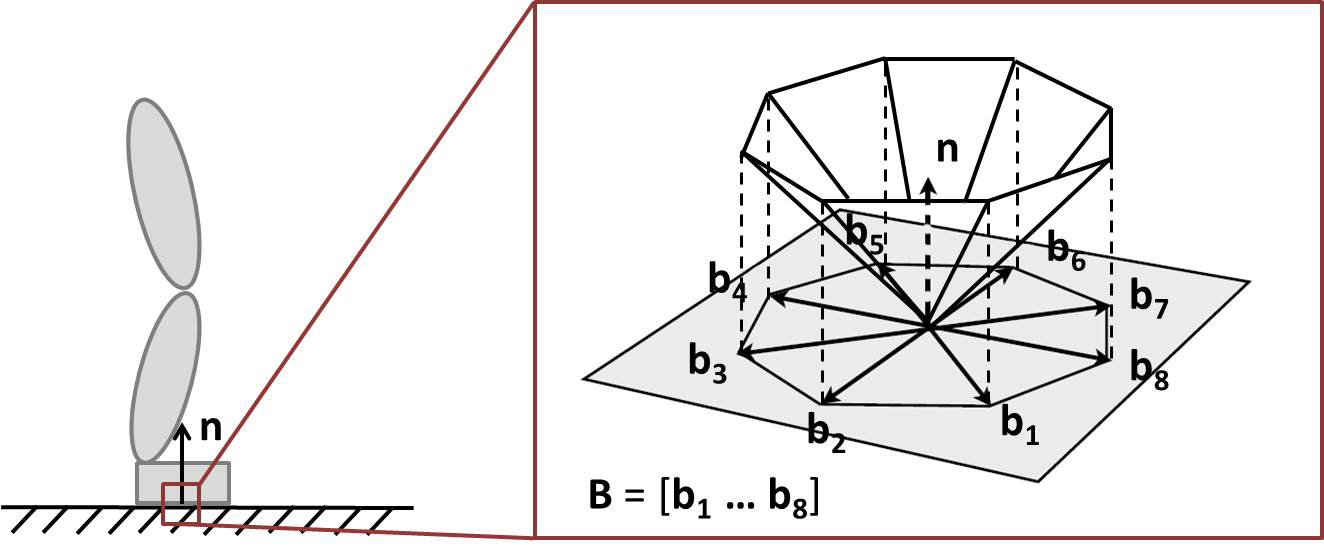
\includegraphics[width=0.85\textwidth]{figures/contact.jpg}
  \caption{A linearized friction cone used in LCP formulation. Left: a foot is in contact with the ground. Right: the friction cone at the contact point. $\vc{n}$ is the contact normal, and $\vc{b}_i$ are a set of tangential bases.}
  \label{fig:contactCone}
\end{figure}

Linear Complementarity Problem (LCP) is a more accurate and stable method to model contacts. A contact force $\vc{f}_c$ can be decomposed into the normal and the tangential (frictional) forces.
\begin{displaymath}
\vc{f}_c = f_\perp\vc{n}+\vc{B}\vc{f}_{\parallel}
\end{displaymath}
where $\vc{n}$ is the contact normal, $f_\perp$ and $\vc{f}_{\parallel}$ are the normal and tangential components respectively. $\vc{B}$ is a set of bases that span the tangential plane (Figure ~\ref{fig:contactCone}). The more basis $\vc{b}_i$ are used, the more accurate approximation of the friction cone is, but more computation is needed to solve the resulting LCP. 

LCP imposes a set of constraints to satisfy the conditions of Coulomb friction: 1) In the normal direction, only repulsive forces are exerted to stop penetration. 2) In the static contact situation, the contact force lies within the friction cone. 3) In sliding contact situation, the contact force lies at the boundary of the friction cone and the friction direction is opposite to the sliding direction. I will illustrate the concept of LCP using the formulation in the normal direction. The formulation in the tangential directions is beyond the scope of this chapter. It can be found in the following tutorials \cite{Lloyd:2005,Tan:2012b}. 

In a physical simulation, after the collisions are resolved, the relative velocity between the contact points of two colliding bodies can only be either zero (resting) or positive (separating), but not negative (penetrating):
\begin{equation}
v_\perp\geq 0
\label{eq:separating}
\end{equation}
Similarly, the normal contact force can be zero (no force) or positive (repulsive force), but not negative (sticking force):
\begin{equation}
f_\perp \geq 0
\label{eq:repulsive}
\end{equation}
The repulsive normal force exists ($f_\perp>0$) if and only if the two bodies are in contact ($v_\perp=0$). In contrast, when they are separating ($v_\perp>0$), there is no contact force ($f_\perp=0$).
In other words, the following linear complementarity condition needs to be satisfied:
\begin{equation}
v_\perp f_\perp =0
\label{eq:complementarity}
\end{equation}

Combining the dynamics equations (eq. \ref{eq:dynamics} or ~\ref{eq:generalized}) and the LCP constraints (eq. \ref{eq:separating}, \ref{eq:repulsive}, \ref{eq:complementarity}) forms a mixed LCP problem. It be solved efficiently by direct \cite{Lloyd05} or iterative solvers \cite{Erleben:2007,Kaufman:2008,Otaduy:2009}. 


\subsection{Simulation Software}

There is a growing need for simulation software that can accurately simulate the complex dynamics of virtural humans and their interactions with their surrounding environment. A couple of open source physical simulators are readily available for research in physically-based character animation. The popular ones include Open Dynamic Engine (ODE) \footnote{http://www.ode.org/}, Bullet \footnote{http://www.bulletphysics.org/}, Dynamic Animation and Robotics Toolkit (DART) \footnote{http://dartsim.github.io/} and MuJoCo \footnote{http://www.mujoco.org}. All of them can simulate articulated rigid bodies with an LCP-based contact model in real time. These simulators allow the user to specify the structure of the articulated figure, the shape and the physical properties of each body, the type of joints, and other parameters describing the environment. Different simulators may offer different features, speed and accuracy. \citet{ErezTT15} provide an up-to-date review and an in-depth comparison among these modern physical engines.
